\section{Opis reaktora polimeryzacji}
Do badań został wykorzystany reaktor polimeryzacji. Jest on schematycznie przedstawiony na rysunku \ref{fig:schemat_reaktor}.
\begin{figure}[H]
	\centering 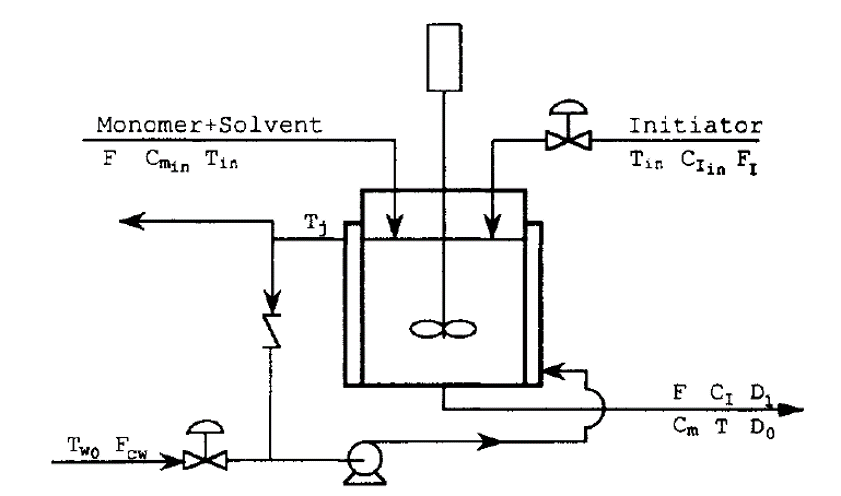
\includegraphics[width=0.8\linewidth]{schemat_reaktor.png}
	\caption{Schemat reaktora polimeryzacji}
	\label{fig:schemat_reaktor}
\end{figure}
Opisany jest on następującymi równaniami stanu:
\begin{equation}
\begin{split}
\dot{x}_1 &= - \left[Z_P\exp\left(\frac{-E_P}{RT}\right) + Z_{f_m}\exp\left(\frac{-E_{f_m}}{RT}\right)\right]x_1P_0(x_2, T) - \frac{Fx_1}{V} + \frac{FC_{m_{in}}}{V} \\
\dot{x}_2 &= - Z_I\exp\left(\frac{-E_I}{RT}\right)x_2 - \frac{Fx_2}{V} + \frac{f_IC_{I_{in}}}{V} \\
\dot{x}_3 &= \left[0.5Z_{T_C}\exp\left(\frac{-E_{T_C}}{RT}\right) + Z_{T_d}\exp\left(\frac{-E_{T_d}}{RT}\right)\right]P_0^2(x_2, T) + Z_{f_m} \exp\left(\frac{-E_{f_m}}{RT}\right) x_1P_0(x_2, T) - \frac{Fx_3}{V} \\
\dot{x}_4 &= M_m\left[Z_P\exp\left(\frac{-E_P}{RT}\right) + Z_{f_m}\exp\left(\frac{-E_{f_m}}{RT}\right)\right]x_1P_0(x_2, T) - \frac{Fx_4}{V}
\end{split}
\end{equation}
gdzie:
\begin{equation}
P_0(x_2, T) = \left[\frac{2f*x_2Z_I\exp(-E_I/RT)}{Z_{T_d}\exp(E_{T_d}/RT)+\exp(-E_{T_C}/RT)}\right]^{1/2}
\end{equation}
Poszczególne zmienne stanu mają następujące znaczenia:
\begin{itemize}
	\item $x_1 = C_m$
	\item $x_2 = C_I$
	\item $x_3 = D_0$
	\item $x_4 = D_I$
	\item $u = F_I$
	\item $y = \frac{D_I}{D_0}$
	\item $d = C_{m_{in}}$
\end{itemize}
Po podstawieniu parametrów reaktora otrzymujemy następujące uproszczone równania stanu:
\begin{equation}
\begin{split}
\dot{x}_1 &= -10x_1 - 2,4568x_1\sqrt{x_2} + 10d\\
\dot{x}_2 &= - 80u - 10,1022x_2\\
\dot{x}_3 &= 0,0024121x1\sqrt{x_2} + 0,112191x_2 - 10x_3 \\
\dot{x}_4 &= 245,978x_1\sqrt{x_2} - 10x_4 \\
y &= \frac{x_4}{x_3}
\end{split}
\end{equation}
Przedstawiony obiekt został zasymulowany w programie MATLAB za pomocą metedy Rungego-Kutty 4. rzędu z czasem próbkowania $T_s = 0,01h$.